%\documentclass{aastex}
\documentclass[iop]{emulateapj}
\usepackage[utf8]{inputenc}
\usepackage{apjfonts}
\usepackage{multirow}

\usepackage{graphicx}
\usepackage{epstopdf}

\newcommand{\myshorttitle}{Near-IR Imaging of M31}
\newcommand{\myshortauthors}{Sick et al.}

\usepackage{color}
\usepackage[dvipsnames]{xcolor}
\usepackage[pdfauthor={\myshortauthors},pdftitle={\myshorttitle},colorlinks=true,citecolor=blue,linkcolor=blue,urlcolor=blue]{hyperref}
\usepackage{url}

\usepackage{amssymb}
\usepackage{amsmath}

\usepackage{natbib}
\bibliographystyle{apj}

\newcommand{\ie}{\textit{i.e.}}
\newcommand{\eg}{\textit{e.g.}}
\newcommand{\vect}[1]{\boldsymbol{#1}} % vectors or images
\newcommand{\sw}[1]{\textit{#1}} % style software titles
\newcommand{\sn}{\ensuremath{S/N}} % signal to noise
\newcommand{\sersic}{S\'{e}rsic}
\newcommand{\iiwione}{\sw{`I`iwi 1.0}}
\newcommand{\androids}{\textsc{androids}}
\newcommand{\changeit}[1]{\textcolor{red}{#1}} % markup bad sections
\newcommand{\todo}[1]{\textcolor{RedOrange}{#1}} % markup TODOs
\newcommand{\Fig}[1]{Fig.~\ref{fig:#1}}  % figure reference macro
\newcommand{\Eq}[1]{Eq.~\ref{eq:#1}}  % equation reference macro
\newcommand{\Tab}[1]{Table~\ref{tab:#1}}  % table reference macro
\newcommand{\Sec}[1]{\S\ref{sec:#1}}  % section reference macro

% To track draft versions in git
\IfFileExists{vc.tex}{\input{vc}}{}

% aastex setup
\shorttitle{\myshorttitle}
\shortauthors{\myshortauthors}

\begin{document}
    \IfFileExists{vc.tex}{\slugcomment{Version \VCRevision\ by \VCAuthor\ on \VCDateTEX , \VCTime .}
}{\slugcomment{Revision unknown.}}
\title{ANDROIDS I. Near-Infrared Imaging of M31}
\author{Jonathan Sick, Stéphane Courteau and the \androids\ collaboration}
\affil{Queen's University}
\affil{Stirling Hall, Kingston Canada}
\email{jsick@astro.queensu.ca}
% \author{Michael McDonald, Brent Tully, Roelof de Jong}

% ============================================================================
\begin{abstract}
Abstract.
\end{abstract}

% ============================================================================
\section{Introduction}
\label{sec:intro}

Near-infrared (NIR) provides a valuable view into galaxies.
NIR is a segment of the spectral energy distribution (SED) of galaxies that is only recently gaining attention, mostly due to the immaturity of detectors.
NIR, in conjunction with ultraviolet and optical bands, offers a partial remedy for the age-metallicity-dust degeneracy that plague stellar population interpretations. 
Traditionally the NIR has also been treated as a stellar mass map, tracing the low end of the stellar initial mass function with minimal dust obfuscation.
Yet the scientific promise of the near-infrared as not been realized.

\cite{Maraston:1998} pointed out that most of the NIR light from intermediate age populations is contributed by thermally-pulsating asymptotic giant branch stars (TP-AGBs). These TP-AGB stars are notoriously difficult to model and include in spectral synthesis models. As a result, the optical-NIR SEDs of galaxies cannot be consistently modelled \citep{Taylor:2011}. Consequently, the best practise for stellar mass estimation as advocated by \cite{Taylor:2011} is to omit the NIR SED from fits, and rely upon useful stellar population degeneracies that, by coincidence, enforce a $g-i$ vs. $\Upsilon_*$ relation.

One means forward for NIR is improved empirical spectral libraries. 
\todo{Cite X-shooter, other NIR spectral library efforts?}
Another way to understand, and possibly calibrate, the NIR light is to observe nearby galaxies where stellar populations can be robustly understood (with exhaustive SED coverage and resolved stellar populations).
Here the Andromeda galaxy stands as a unique and important telescope.
It is visible to the Northern Hemisphere and thus to the premiere wide-field NIR imager (CFHT/WIRCam), and close enough (785 kpc) that stars can be resolved thoughout the disk without adaptive optics.

\cite{Beaton:2007} assembled a 2.8\arcdeg\ $JHK_s$ mosaic centered on M31 with the 2MASS 6X program.
Those observations, which trace the stellar galaxy mass, were used by \cite{Athanassoula:2006} as evidence of a bar embedded in a classical bulge.
But beyond the bulge, the 2MASS 6X images have limited utility.
\cite{Courteau:2011} find sky uncertainty prevents using the 2MASS 6X to infer structural and photometric properties of the disk.
Further, the pixel scale of 1\arcsec\ and integration depth of 46.8 seconds prevents point source measurements of the 2MASS 6X images.
As a result, the defacto state-of-the-art NIR view of M31 is the slightly longer 3.6 $\mu$m Spitzer/IRAC map of \cite{Barmby:2006}.
Spitzer obviates the issue of sky estimation, although the pixel scale of 0\farcs86 also prevents point source measurements of individual stars in the M31 disk.

In this paper, we present a survey of the M31 bulge and disk with CFHT/WIRCam in the $J$ and $K_s$ bands.
These are the first global near-infrared observations of M31 that simultaneously resolve throughout the mid- and outer-disk, while also recovering attempting to rigorously recover the NIR surface brightness.
While future contributions will explore the resolved near-IR stellar populations, our focus here is the surface brightness calibration of the WIRCam data set, and exploration of NIR sky subtraction uncertainties.
Section~\ref{sec:Observations} describes the novel observational strategies used to reduce sky subtraction uncertainties.
Section~\ref{sec:reduction} describes the image reduction pipeline; a particularly important aspect of this is night sky flat fielding (\S\ref{sec:flats}).
In \S\ref{sec:scalar} we present our method for recovering the galaxy surface brightness by minimizing the image-to-image differences across the mosaic.
We estimate the systematic uncertainties in our mosaic solution in \S\ref{sec:systematics}, where we also compare our technique to the Montage package \citep{Berriman:2008} and the Spitzer/IRAC mosaics.
Finally in \S\ref{sec:conclusions} we summarize the uncertainty of NIR sky subtraction on the scale of M31.

% ============================================================================
\section{Observations}
\label{sec:Observations}

\begin{figure}[t]
	\centering
		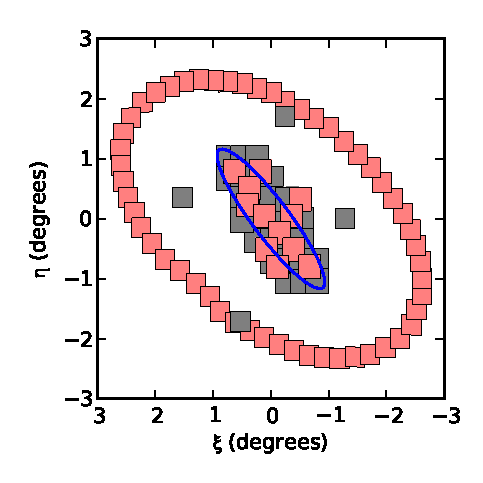
\includegraphics[width=3in]{figs/fieldmap}
	\caption{WIRCam field positions on M31. Grey fields at center at the 27 disk fields observed in 2007B, surrounded by 4 sky fields. Red fields at center are the 12 disk fields observed in 2007B. The red ring of 53 fields is the 2009B sky sampling ring. The blue ellipse marks the M31 disk at $R=20$ kpc along the major axis. Coordinates are centered on the nucleus of M31 with North up, and East towards left.}
	\label{fig:fieldmap}
	% made with skyoffsets/chart.py
    % TODO fix colouring of disk vs sky fields.
\end{figure}

% Surface brightness CI from skyoffset/net_sky_level.py
% Median and 95% C.I.
% 2007B J 15.1195176911 ; 14.9139114767 -- 15.3477818651
% 2009B J dim 14.5613758489 ; 14.2933487068 -- 14.8544020768
% 2009B J bright 15.2006801085 ; 15.1336648803 -- 15.2789519627
% 2007B Ks 13.354737759 ; 13.1811645305 -- 13.6149313145
% 2009B Ks 13.27306929 ; 13.1173594814 -- 13.4222534742

\begin{table*}[t]
    \caption[Summary of WIRCam observing programs]{Summary of WIRCam observing programs. ST Nods are coded with superscripts to denote the number of times an observation is repeated at a given field. Efficiency (Eff.) is the percentage of time in a program allocated to integrating the disk of M31, compared from nodding, read out and sky overheads. Seeing is measured from stars in sky images.}
    \label{tab:obssummary}
    
    \centering
    \begin{tabular}{lllllllllll}
        & & & & $\frac{T_\mathrm{int}}{\mathrm{field}}$ & $T_\mathrm{exp}$ & Eff. & $\mu_\mathrm{sky}$ 95\% C.I. & \multicolumn{3}{c}{PSF FWHM (arcsec)} \\ \cline{9-11}
    Semester & Band & $N_\mathrm{disk}$ & ST Nods & (min) &  (s) &  (\%) & (mag/arcsec$^2$) & 25th  & 50th & 75th \\
    \hline
    \multirow{2}{*}{2007B} & $J$ & \multirow{2}{*}{27} & [S$^3$T$^8$S$^3$]$^{2}$S$^3$ & 12.5 & 47 & 49 & (14.9, 15.3) & 0.68 & 0.75 & 0.84 \\
     & $K_s$ &  & [S$^5$T$^{13}$S$^5$]${^2}$S$^5$ & 10.8 & 25 & 42 & (13.2, 13.6) & 0.60 &  0.65 & 0.73 \\
     \hline
     \multirow{2}{*}{2009B} & $J$ & \multirow{2}{*}{12} & \multirow{2}{*}{[ST$^2$S]$^{20}$S} & \multirow{2}{*}{13.3} & \multirow{2}{*}{20} & \multirow{2}{*}{26} & (14.3, 14.6), (15.1, 15.3) & 0.61 & 0.69 & 0.83 \\
      & $K_s$ & & & & & & (13.1, 13.4) & 0.60 & 0.66 & 0.76 \\
    \end{tabular}
\end{table*}

% \begin{deluxetable}{10}
% % \tabletypesize{\small} % or \footnotesize or \scriptsize
% % \rotate
% % \tablewidth{⟨dimen ⟩}
% % \tablenum{⟨text ⟩}
% \tablecolumns{⟨num ⟩}
% \tablecaption{Summary of WIRCam observing programs. Efficiency (Eff.) is the percentage of time in a program allocated to integrating the disk of M31, compared from nodding, read out and sky overheads. Seeing is measured from stars in sky images.
%     \label{⟨key ⟩}}
% \tablehead{⟨text ⟩}
% \end{deluxetable}

The Andromeda Galaxy (M31) was observed in the NIR using the WIRCam instrument, mounted to the 3.6-meter Canada-France-Hawaii Telescope (CFHT), at the summit of Mauna Kea in Hawaii. Observations were carried out exclusively in the NIR $J$ ($\lambda_0 \sim 1.2 \mu\mathrm{m}$) and $K_s$ ($\lambda_0 \sim 2.2 \mu\mathrm{m}$) bands.

WIRCam itself is an array of four HgCdTe HAWAII-RG2 detectors \citep{Puget:2004}. Each detector comprises $2048\times 2048$ pixels, with a scale of 0\farcs 3 . This pixel scale critically samples the typical seeing of 0\farcs 65 seen by CFHT. For reference, $1\arcsec = 3.7~\mathrm{pc}$ across the disk of M31. The detectors are arranged in a $2\times 2$ grid with 45\arcsec\ gaps, so that the entire instrument covers $21.5\arcmin \times 21.5\arcmin$ of sky. It is truly the recent advent of NIR focal plane arrays, like WIRCam, that have enabled relatively efficient studies of M31 in the NIR.

The \androids\ WIRCam survey is designed to simultaneously resolve stars and recover the integrated surface brightness of the M31 disk. While the former objective is attained by requesting good seeing in Queued Service Observing mode (see Table \ref{tab:obssummary}), WIRCam has not previously been used to recover surface brightness at the accuracy required---$\mu_{K_s}\lesssim~22$~mag~arcsec$^{-2}$---across entire detector fields. As discussed in \S \ref{sec:intro}, NIR observations require frequent monitoring of the sky background. Since M31, with a $190\arcmin \times 60\arcmin$ optical disk, is much larger than the WIRCam fields of view, monitoring of the sky zeropoint is only possible by periodically pointing the telescope away from M31, towards blank sky---\emph{sky-target} (ST) nodding. 

Observations were taken over two semesters, 2007B and 2009B. The two campaigns employed different observing schemes, particularly sky-target nodding strategies. The reader is encouraged to regard these observational designs as \emph{hypotheses} for how to best conduct a wide-field surface brightness survey in the near-infrared from the ground. An objective of this paper is to discriminate between the virtues of the 2007B and 2009B programmes, and determine if observational design can improve the construction of a wide-field NIR mosaic.

\begin{figure}[t]
    \centering
        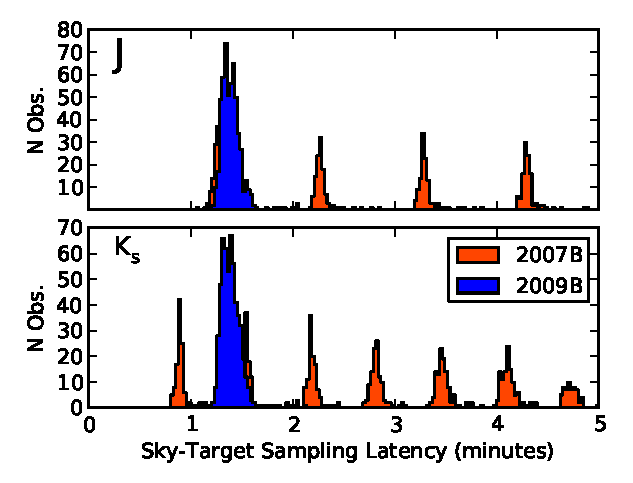
\includegraphics[width=3in]{figs/sky_target_lag}
    \caption{Time latency between target observations and sky field sampling in the 2007B and 2009B WIRCam observing runs. The 2009B program was designed to ensure that no disk sample would be removed by more than 1.5 minutes from a sky sample by using a STTS nodding pattern.}
    \label{fig:sky_target_lag}
    % made with skyoffsets/obs_run_stats.py
\end{figure}

\begin{figure}[t]
    \centering
        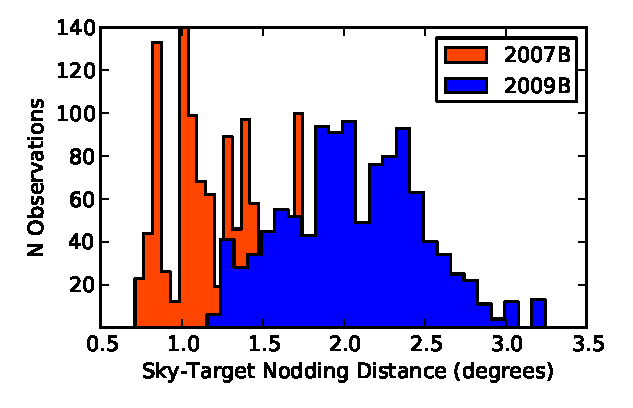
\includegraphics[width=3in]{figs/sky_target_dist}
    \caption{Distance between sky and target observations in the 2007B and 2009B WIRCam observing runs. The larger nodding distance of 2009B is a consequence of sky ring sampling. The maximum nodding distance across the sky ring was purposefully set to $\sim 3$\arcdeg\ to avoid excessive time overheads. As such, a given disk field only samples roughly of the full sky ring.}
    \label{fig:sky_target_dist}
    % made with skyoffsets/obs_run_stats.py
\end{figure}

\begin{figure}[t]
    \centering
        \includegraphics[width=3.25in]{figs/sky_level_hist}
    \caption{Sky levels observed in the 2007B (red outline) and 2009B (grey filled) programs.}
    \label{fig:net_sky_level}
    % made with skyoffset/net_sky_level.py
\end{figure}

\subsection{2007B Semester} % (fold)
\label{sec:obs7}

The initial survey was carried out in the 2007B semester by the CFHT Queue Service Observing under photometric conditions. This programme covers M31 with 27 contiguous WIRCam fields covering the entirety of M31 out to the optical radius: $\mu_V=23$ mag arcsec$^{-2}$, $R=20$~kpc. The fields are arranged with at least 1\arcmin\ overlap in declination, and approximately 5\arcmin\ overlap in right ascension.
% FIXME check overlaps
This arrangement yields a continuous mosaic that avoids masked pixels that obscure the eastern 3\arcmin\ of the WIRCam array. The field configuration is shown in Fig. \ref{fig:fieldmap}.

Each field was integrated for $16\times 47 s = 12.5$ minutes in $J$ and $26\times 25 s = 10.8$ minutes in $K_s$. These integrations are sufficiently deep for resolved stellar photometry to reach at least 1 mag below the tip of the red giant branch, a crucial requirement for decomposing the contributions of red giant and asymptotic giant branch stars to the NIR light. \changeit{Superfluous for a SB paper?}

The 2007B ST nodding strategy was motivated by a canonical understanding of NIR sky behaviour, since ST nodding sky subtraction had never been attempted on this scale before. The NIR sky intensity can be expected to change by 5\% in 10~minutes \citep{Adams:1996,Vaduvescu:2004}; since the sky itself is 5~dex brighter than the outer disk of M31 in the NIR, a 5\% uncertainty in the background would be fatal to our objective of recovering M31's NIR surface brightness. To constrain the sky to within 1\%, we chose to monitor the sky so that at worst, a sky sample would be no more than 5 minutes removed from a M31 target image. Given the exposure times, this implied a sky (S)--target (T) observing sequence of $S^3T^8S^3$ in $J$ and $S^5T^{13}S^5$ in $K_s$.\footnote{Superscripts here denote the number of times an observation is repeated in sequence for a given target disk field.} Four sky fields were chosen (Fig \ref{fig:fieldmap}), and each disk field was associated with a single sky field.

% subsection obs7 (end)

\subsection{2009B Semester} % (fold)
\label{sub:obs9}

Initial analysis data set revealed that the canonical sky-target nodding strategy of the 2007B campaign was not sufficient for recovering the M31 surface brightness due to uncertainties in the sky background. This motivated a 2009B observing campaign informed by our experiences.

Rather than replicate the 28-field footprint of the 2007B campaign, we observed 12 fields. These fields overlap each other, and all of the 2007B footprints, to form a network of well-sky subtracted fields. That is the 2009B observations augment and calibrate the 2007B NIR mapping.

To improve sky subtraction fidelity, we recognized challenges not fully appreciated in the 2007B survey design. Not only does the sky background change rapidly in time, it possess a significant spatial structure on the scale of WIRCam fields and larger. This has two ramifications: the sky level sampled at a sky field \emph{will not} necessarily reflect the sky background present at the disk, and that the sky background in each WIRCam frame has a 2D shape, not simply a scalar level.

This resulted in three principle changes to observing strategy. First, we chose to minimize latency between sky and target observations with a ST$^2$S pattern. That is, each target observation was directly paired with a sky observation taken within 1.5 minutes (Fig. \ref{fig:sky_target_lag}).

Second, we also increased the number of repetitions on each field, so that each field is observed 40 times in each band in a [ST$^2$S]$^{20}$S pattern. This repetition permits the opportunity to average over spatial sky background structures on the scale of WIRCam fields.

Finally, we employ an innovative randomized sky-targeting nodding pattern where no sky field is used repeatedly for a disk field. In order to maintain rapid telescope nods, only northern sky fields serviced the northern disk, and similar for the southern fields; the maximum offset on the sky was 3\arcdeg\ (see Fig. \ref{fig:sky_target_dist}). This random sampling of sky fields yielded two possible advantages: 1) when a median sky image is constructed, many \emph{sky shapes} are combined, possibly yielding an intrinsically flatter image of sky (see \S on median sky subtraction), and 2) if there is a coherent structure in the NIR sky, sampling fields of the sky degrees apart in rapid succession should average out these systematic biases in estimating the sky level \emph{on the disk}.

% subsection obs9 (end)

% ============================================================================
\section{Image Preparation}
\label{sec:reduction}

Our goal is to produce an accurate mosaic of M31 from ground-based, CFHT/WIRCam, NIR images.
%Here we wish to comment on some of the image reduction steps that have a significant impact on the quality of our final mosaic, and the custom WIRCam pipeline adaptation made by \androids.
Central to this paper, then, is the development of best practises for reducing CFHT/WIRCam images and mapping surface brightness with a sky-target nodding observing scheme on a target as large as M31.
The objectives of this paper require us to significantly exceed the observational performance of WIRCam realized by other studies.
To realize this performance, we must carefully analyze each step of the reduction process, including flat fielding, photometric calibration and sky subtraction.
The product of this paper is a novel pipeline for reducing CFHT/WIRCam data that is outlined next in \S\ref{sec:reduction_outline}, and in subsequent sections.

WIRCam data are offered by CFHT in three progressive stages of \emph{preprocessing} by their \iiwione\ pipeline to allow programmes, such as this one, to re-implement calibration recipes for potentially higher performance.
These data flavours are: a raw image that is essentially untouched after leaving the instrument (\texttt{*o.fits}); an image that has been nonlinearity-corrected, dark subtracted and flat fielded (\texttt{*s.fits}); and an image that has been sky subtracted, in addition to all the previous treatments (\texttt{*p.fits}).

As sky subtraction is the highest source of error in this program, the middle data product, \texttt{*s.fits}, would appear most amenable as a starting point for this program.
Nonetheless, two \iiwione\ processing stages included in \texttt{*s.fits} products must be handled carefully.

\paragraph{Cross-talk correction} WIRCam integrations prior to March 2008 (that is, the 2007B data set, but not the 2009B data) suffered from electronic cross talk within the detector.
This cross talk is manifested in repeating rings above and below saturated stars.\footnote{See \url{http://cfht.hawaii.edu/Instruments/Imaging/WIRCam/WIRCamCrosstalks.html}.}
By default, the \iiwione\ pipeline removes this cross talk by subtracting a median of the 32 amplifier slices.
Unfortunately, this algorithm fails in cases where the background has a surface brightness gradient (such as on the disk of M31) and produces an inverse surface brightness gradient that is stronger than the galaxy surface brightness itself.
Loic Albert was kind to re-process the 2007B data set with the cross-talk correction turned off.

\paragraph{Flat fielding} We discovered that the dome flat fielding offered by \iiwione\ was only accurate to 2\% of edge-to-edge intensity.
The ineffectiveness of WIRCam dome flat fielding is evident in \texttt{*s.fits} images that show significant detector structure, despite having been flat fielded.
An example of this structure is related to the different gain structures of the 32 amplifiers that service independent horizontal bands across each WIRCam detector (see Fig \todo{TODO})---a proper flat field must be able to capture such gain structure for proper photometry.
Users of fully-processed \iiwione\ \texttt{*p.fits} images do not directly notice the unsuitability of dome flats since images of the detector gain structure embedded in the NIR bright sky background are \textit{subtracted} from the signal as part of the median sky subtraction step.
Yet since pixel gain changes the signal in proportion to incident flux, subtraction is fundamentally the wrong operation to use.
Our remedy is to adopt night sky flats, which use the median night sky as the illumination reference rather than a dome lamp.
Comparing the dome and night sky flats, as in \Fig{domeflatratio}, shows how profound the choice of flat field can be.
Our confidence in night sky flats as the \textit{correct} choice for flat fielding WIRCam lays in its ability to remove both large scale illumination features and pixel-to-pixel gain changes across WIRCam (see Fig \todo{TODO}).
But the production of WIRCam sky flats is subtle as we find the gain structure of WIRCam to be time dependent on scales of hours, and of course the NIR night sky itself is not flat.
A comprehensive discussion of WIRCam flat fielding is made in \S~\ref{sec:flats}.

\begin{figure}[t]
   \centering
    \includegraphics[width=3in]{figs/flatratio_09BQ01_Ks_twocol}
    \caption{Percent difference image of the 09BQ01 $K_s$ (queue run) sky flat to the \texttt{domeflat\_8302B\_20090728HST143302\_Ks} dome flat used in the \iiwione\ pipeline. Using the median night sky illumination over a WIRCam queue run, rather than a dome lamp, results not only in 2\% edge-to-edge different in the large scale WIRCam illumination function, but also in different characterizations of gain structure in the WIRCam detector amplifiers (the 32 horizontal bands in each of the four WIRCam detectors).}
   \label{fig:domeflatratio}
   % made with skysubpub/flatratio.py
\end{figure}

\vspace{1em}

Our \androids\ pipeline thus begins with \texttt{*s.fits} data that have been undone of flat fielding.
That is, we multiply the \texttt{*s.fits} image with with its associated dome flat.\footnote{Dome and twilight flats are made available by CFHT, \url{http://limu.cfht.hawaii.edu:80/detrend/wircam/}.}
The result is an image that retains \iiwione's prescription for dark subtraction, bad pixel masking and non-linearity correction.
The \androids\ WIRCam pipeline then carries out steps described here, and in the following sections.

\subsection{Reduction outline}
\label{sec:reduction_outline}

Our ANDROIDS/WIRCam reductions begins by unifying the World Coordinate System across the dataset with \sw{Scamp} \citep{Bertin:2006}.
Scamp matches stars in Source Extractor \citep{Bertin:1996} catalogs of each WIRCam \texttt{*p.fits} frame both internally (to \todo{TODO} \arcsec ), and against the 2MASS Point Source Catalog (\todo{CITE}) to a precision of \todo{TODO}\arcsec .
So that all frames match field-to-field and between $J$ and $K_s$ bands, astrometric solutions for all \todo{TODO} frames of the ANDROIDS/WIRCam survey are assembled simultaneously.  Scamp handles this data volume gracefully provided we cull the input star catalogs for stars of $S/N > 100$, and by using the \texttt{SAME\_CRVAL} astronometry assumption that the WIRCam focal plane geometry is stable.

In parallel, we apply flat fields constructed from sky signal in the \textit{deflattened} \texttt{*s.fits} images.
Sky flats produced the observations themselves are able to track gain variations across the WIRCam detectors throughout the night.
These flat fielded images still possess a sky background illumination that must be estimated and subtracted.
This can done by constructing \textit{median sky frames}, median combinations of five sequential sky 
images.
This procedure was originally motivated by near-infrared programs where the objects are small, so that the median of several frames in a multi-point dither pattern effortlessly removes the signal flux, leaving only an image of the sky background itself.
An advantage of median sky construction is that it not only records the amplitude of a sky signal, but also its \emph{shape}.
For large sky-target nods, the recorded shape of the sky will be a less relevant representation of the sky on the target itself.
Nonetheless, \iiwione\ retained this practice of median sky construction as a crutch for removing instrumental signals not removed by dome flat fielding (see \S~\ref{sec:flats}). In this ANDROIDS pipeline we find that even sky flat fielding leaves a background shape that persists across sky fields, and that must be subtracted with median sky subtraction.
Discussion of sky flat and median sky subtraction construction is saved for \S~\ref{sec:flats} where we argue the appropriate time window for averaging sky flux into a sky flat field, and the shapes of residual sky captured by median sky subtraction. \todo{(Fix sentence)}

These flat fielded and background subtracted frames are photometrically calibrated to a uniform zeropoint.
We cannot use the CFHT \iiwione\ zeropoints because of our custom sky flat fielding; zeropoints are instead estimated against 2MASS stars in the WIRCam fields.
The photometric calibration, including colour transformations between the CFHT/WIRCam and 2MASS filters are discussed in the next section (\S~\ref{sec:photcal}).

Finally, while the data has formally been flat fielded and photometrically calibrated, the sky level estimation provided by the sky-target nodding observing scheme is not accurate enough to build a seamless mosaic.
Instead we model sky offsets that enforce internal consistency in the sky levels of target frames.
In \S~\ref{sec:scalar} we discuss the methods for modelling these sky offsets and their analyze their amplitudes.

\section{Sky Flat Fielding}
\label{sec:flats}

Dome flats fail to properly calibrate WIRCam data, as evidenced by Figs.~\ref{fig:domeflatratio} and \todo{TODO}.
Sky flats are an appropriate alternative, both because of the of the abundant sky background (any NIR imaging program can use its own images to build sky flats), and because sky flats more aptly trace detector illumination and gain structure.
The former because skylight traces the same optical path as astronomical sources; the latter because WIRCam's gain structure appears variable.
Sky flats allow detector gain mapping in real-time.
We return to the subject of WIRCam's variable gain structure later in this section.

\subsection{Building Sky Flats}
\label{sec:flatbuilding}

Producing sky flat is principally as simple as median combining integrations of blank sky. 
The \androids\ sky-target nodding observing strategy provides an abundance of `sky' images for this purpose.
A fundamental decision is to define the window of sky integrations to be combined into a sky flat.

One choice is to assume that flat fields are stable over a queue run (a continuous installation period of WIRCam).
In this case, all sky integrations taken during a queue run, and through a given filter, are combined into what we denote as a `QRUN Sky Flat.'
This choice is reasonable since dust and optical geometry should be stable during a continuous mounting period.
Further, choosing a large pool of sky images ensures high \sn\, and helps to helps to marginalize over the shape of the sky background.
Table~\ref{tab:flattable} lists statistics of the QRUN sky flats.

\begin{table}[t]
\centering
\caption{Properties of night sky flats constructed for each Queue Run (\texttt{QRUNID}).}
\label{tab:flattable}

\begin{tabular}{cccc}
\hline
Filter & QRUNID & $N$ images & $N$ nights \\
\hline
$J$ & 07BQ01 & 24 & 6 \\
$J$ & 07BQ03 & 141 & 9 \\
$J$ & 07BQ05 & 43 & 4 \\
$J$ & 09BQ01 & 111 & 10 \\
$J$ & 09BQ03 & 55 & 3 \\
$J$ & 09BQ08 & 396 & 10 \\
\hline
$K_s$ & 07BQ01 & 35 & 2 \\
$K_s$ & 07BQ03 & 25 & 1 \\
$K_s$ & 07BQ05 & 156 & 6 \\
$K_s$ & 07BQ07 & 133 & 3 \\
$K_s$ & 09BQ01 & 113 & 10 \\
$K_s$ & 09BQ03 & 55 & 3 \\
$K_s$ & 09BQ08 & 637 & 8 \\
\hline
\end{tabular}
\end{table}

An alternative, more defensive, choice is to assume that WIRCam's illumination function and detector gain structure is unstable even over short periods.
Here the objective is to make many sky flats that reflect the real-time flat field function---we call these Real-Time Sky Flats.
We've chosen to RT sky flats such that the pool of sky images contain cumulative sky levels of at least 100,000 ADU, or that the time span from first to last sky integration be no longer than two hours.
In \Fig{fw100k_membercount} we consider the properties of such real-time sky flats.
$J$-band sky flats typically require 15 integrations during the 07B campaign, or 10--25 integrations in the 09B campaign $J$-band sky levels were bimodal (see \Fig{net_sky_level}).
Given the 07B $J$-band ST nodding pattern, 15 sky integrations are accumulated in 50 minute windows; whereas the more frequent nodding in the 09B campaign shortened this window to 20 minutes (but as long as 50--90 minutes in dark sky conditions).
The brighter $K_s$ sky calls for just 7--13 integrations in 07B, or 10--20 integrations in the 09B campaign.
This number of $K_s$ sky samples was accumulated within 10--30 minutes in 07B, or 10--70 minutes in 09B.
\todo{Redo this plot to incorporate 1) total flux 2) number of sky images, and 3) window span. Remove sky flats associated with the staring fields, and with 11B.}

\begin{figure}[t]
\centering
\includegraphics[width=\columnwidth]{figs/fw100k/member_count}
\caption{Numbers of sky images in real-time sky flats, meeting criteria of at least 100,000 sky ADU, and spans of less than two hours.}
\label{fig:fw100k_membercount}
\end{figure}

Given the ensemble of sky integrations, our next task is to normalize the illumination in each sky image.
We also want to normalize the zeropoints of the four WIRCam detectors.
This scaling is calibrated by the modal pixel level measured on each detector for each sky integration---denote these modal levels as $\alpha_{i,j}$ for the $i$th sky image's level in detector $j$, $j=1, 2, 3, 4$.
Modal sky level measurements are aided by sensitive Source Extractor object masks generated from \iiwione\ \texttt{*p.fits} images (which may be mis-calibrated, but provide valuable clean images of sources).
For each detector, we compute the median sky level seen by that chip: $\beta_j = \mathrm{median}(\alpha_{1,j}, \alpha_{2,j}\ldots \alpha_{n,j} )$.
Each sky image in detector $j$ is then scaled by the factor $median(\beta_1, \beta_2, \beta_3, \beta_4) / \beta_j$.

\section{(Old) Sky Flat Fielding}

Images flat-fielded by \iiwione\ show a remarkable amount of fixed structure.
In most applications of WIRCam, these detector illumination structures are un-noticed since the median sky subtraction step, to produce the `fully pre-processed' \texttt{*p.fits}, will erase these illumination artifacts from blank sky.
That is, median sky subtraction is treated as a secondary flat-field treatment.
However, this is a dangerous procedure as illumination corrections must be multiplicative (as it is a correction to the relative efficiency of detecting photons across the WIRCam detector).
Employing median sky subtraction only removes observed background signal; it does not correct the efficiency of detecting signal across the detector.

The error introduced by dome flat fielding in the \iiwione\ pipeline may be realized by producing a median stack of sky images (\ie, the same procedure to make sky flats) that have been flat fielded by \iiwione\ preprocessing.
While astrophysical sources are eliminated in a median stack, a residual detector structure is revealed that appears to be consistent across WIRCam integrations over time scales of months and years.
These structures can be categorized as a detector-scale illumination variation, distinct patches hundreds of pixels across, and horizontal banding that appears to coincide with the 32-pixel high amplifier bands.

\changeit{The flat field is also effected by what looks like a 2D pixel gain variation that changes on the order or 0.5\% in a few hours. JCC also detects this. This suggests that sky flats should be made with images windowed within 1 hour, rather than an entire QRUN, as suggested in the thesis.}

We attribute the residual unflatness of \iiwione\ preprocessed products to its use of dome flats.
The light path and colour of a reflected tungsten lamp,\footnote{CFHT \iiwione\ manual: \url{http://www.cfht.hawaii.edu/Instruments/Imaging/WIRCam/IiwiVersion1Doc.html}} rather than photons originating from the atmosphere, yields a remarkably different detector illumination calibration.
For this project we chose to redo the flat fielding using \emph{sky flats}: flat field images that use the abundant near-infrared sky signal to describe the illumination function of the WIRCam detectors.
The procedure for building a sky flat is listed in \S\ref{sec:skyflatpro}.

\subsubsection{Construction of night sky flat fields}
\label{sec:skyflatpro}

Sky flats are made from ensembles of sky field images that have been un-done of \iiwione\ dome flat fielding.
We group images into sets of common filer ($J$ or $K_s$), detector (1--4 in WIRCam array) and WIRCam run ID (\texttt{QRUNID}).
We presume that the telescope and electronic signatures are stable over these camera mounting periods.
Table \ref{tab:flattable} lists the number of images grouped into each sky flat.

The ensemble of sky images being combined into a single sky flat have different illumination levels. Thus each frame is scaled (multiplicatively) so that each has a common median value in its central $400\times400$ pixel region.

For each frame, we also build masks for any pixels that do not sample blank sky. \sw{Source Extractor} \citep{Bertin:1996} is used to define stars and background galaxies, while hand-drawn polygon regions cover diffraction spikes and the diffuse halos around bright galactic stars. A third mask is algorithmically produced to cover persistence signals from preceding exposures. These masks, along with the \iiwione\ bad pixel mask, are combined with \sw{WeightWatcher} \citep{Marmo:2008}.

The flat itself is built by median combination. Median combination of a stack of hundreds of $2048\times2048$ pixel image, each with a weightmap, is computationally expensive. A convenient solution was to use \sw{Swarp} \citep[an image-mosaicing software package,][]{Bertin:2002} in a mode that combined images pixel-to-pixel. These median combined frames were normalized to unit mean intensity.

Table \ref{tab:flattable} lists the sky flats constructed for this survey. These sky flats were divided from each sky and disk frame taken under the same conditions (filter, detector and camera installation) to create an illumination-corrected data set.


\subsection{Sky flat performance}
\label{sec:skyflatstats}


\subsubsection{Comparison to \iiwione\ dome flats}

To illustrate the disagreement between the sky and \iiwione\ dome flats, Fig. \ref{fig:domeflatratio} shows a percent difference map of a \iiwione\ dome flat to a sky flat produced via the procedure in \S \ref{sec:skyflatpro}. This map reveals a $\pm2\%$ discrepancy between the two types of flat fields.
% FIXME see thesis/flatratio.py and thesis_plots/ for the flat ratio image.
% In Ks I do see 2\% -- 4\% edge-to-edge.
% TODO repeat this for both $J$ and $K_s$ sky flats.
In practice, the sky flat appears to be the correct description of the WIRCam illumination as application of sky flats \emph{does} remove all types of residual WIRCam illumination features: large scale, small scale, and amplifier band structures.

\subsubsection{Flatness of sky flats}
\label{sec:skyflatshapes}

\begin{figure}[t]
    \centering
        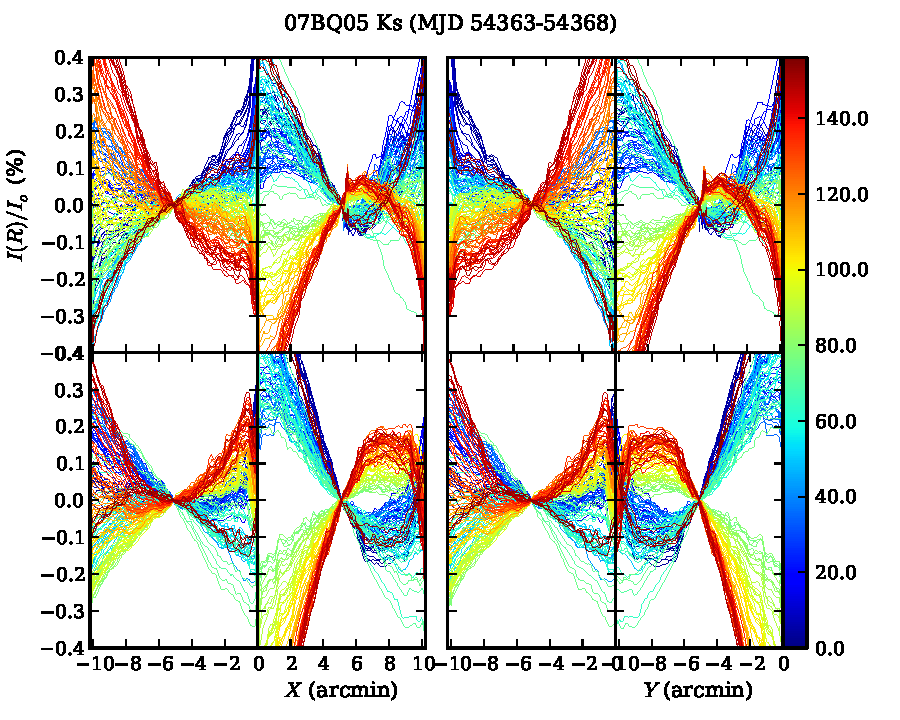
\includegraphics[width=3in]{figs/07BQ05_Ks.pdf}
    \caption{Evolution of the shapes of sky images composed in the 07BQ05 $K_s$ sky flat. Shape is measured as the median trend across the columns (left array) and rows (right array) WIRCam images. These trends are normalized to the level at the centre of the detector, $I_o$. Axes are arranged to match the $2 \times 2$ configuration of WIRCam. Colours highlight the observation sequence of images.}
    \label{fig:flat_07BQ05_Ks}
    % flatshapes.py
    % need to import code used to generate this type of plot
    % TODO label the colourbar as "Sky Image Index", note that its ordered
    % but not necessarily time proportional
\end{figure}

%\begin{figure}[t]
%	\centering
%		\includegraphics[width=\textwidth]{figs/flat/09BQ08_Ks.pdf}
%	\caption[Sky shape composition of 09BQ08 $K_s$ sky flat]{Sky shape composition of 09BQ08 $K_s$ sky flat. See Fig. \ref{fig:flat_07BQ05_Ks} for explanation.}
%	\label{fig:flat_09BQ08_Ks}
%	% flatshapes.py
%\end{figure}

\begin{figure}[t]
   \centering
       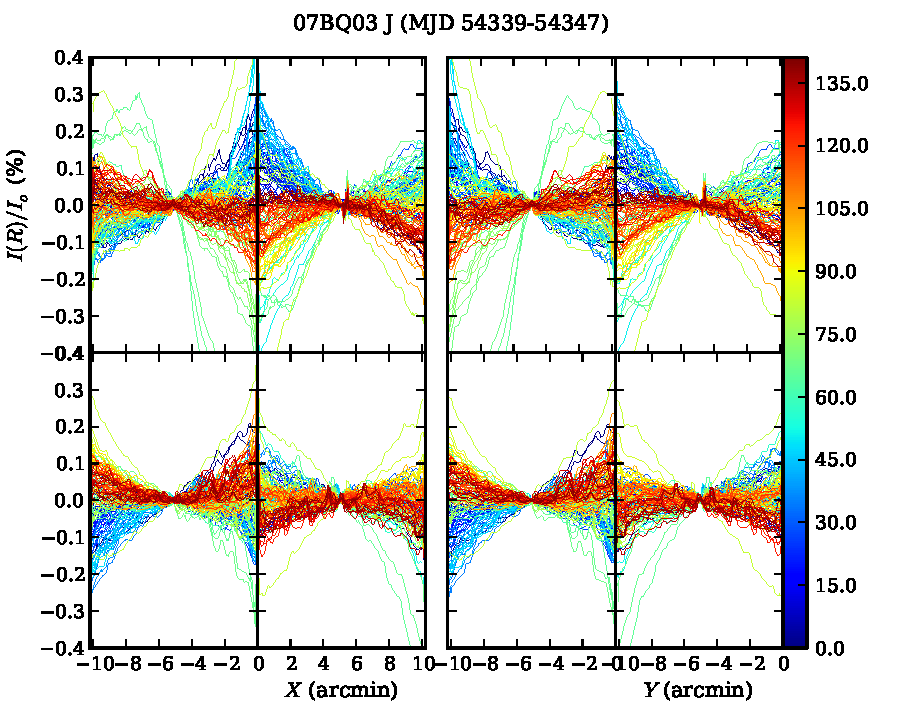
\includegraphics[width=3in]{figs/07BQ03_J.pdf}
   \caption[Sky shape composition of the 07BQ03 $J$ sky flat]{Sky shape composition of the 07BQ03 $J$ sky flat. See Fig. \ref{fig:flat_07BQ05_Ks} for explanation.}
   \label{fig:flat_07BQ03_J}
   % flatshapes.py
\end{figure}

\changeit{TODO: This section needs to be revised w.r.t. the detection of gain variability across the WIRCam detectors.}

Ultimately, the accuracy of sky flats is limited by the distribution of intrinsic shapes in the NIR sky. Wide-field movies of the near-infrared sky \citep{Adams:1996} show the NIR sky glow to be akin to a moving cloud system. As such, the NIR sky seen by WIRCam is never flat---yet by definition a flat field must necessarily be built from an intrinsically uniform illumination across the telescope focal plane. In producing a NIR sky flat, we hypothesize that the \emph{mean shape} of the NIR sky, over the span of a queue run, is flat.

In Figures \ref{fig:flat_07BQ05_Ks}--\ref{fig:flat_07BQ03_J}, I plot the sequences of sky shapes that are combined to produce a sky flat for typical queue runs of this survey. These `sky shapes' are built by median-compressing the sky images down rows and columns to show the general trend of the sky across $x$ and $y$ image axes. The centre-to-edge shape of the sky, across a 10.4\arcmin\ WIRCam detector, typically varies by 0.1\% in $J$, and 0.5\% in $K_s$. \emph{The performance of dome flats---$\pm2\%$ error relative to sky flats---is worse than the typical uncertainty in shape from a single sky frame.} But the ultimate accuracy of sky flats depends upon the distribution of sky shapes composed in a QSO run. And surprisingly, the shapes are not always randomly distributed, in part because of the sporadic bursts of sky observations throughout a queue run, as the CFHT queued observing program balances several difference observing projects at once.

For example, in 07BQ05 ($K_s$) (Fig. \ref{fig:flat_07BQ05_Ks}), we see distinct traces of sky shapes that correspond to the sporadic activation of this observing program over several nights, for 30 minutes to hours at a time (as is the normal structure of queued observing blocks). Over the span of an \emph{observing block}, the sky will vary slowly. Once the sky is observed again on a different night in a queue run, the sky shape will be vastly different, creating the two distinct sets of shapes. In other cases where more observations are made under different sky conditions, such as 09BQ08 ($K_s$), a more continuous set of sky shapes is observed. In the $J$ band (\eg, Fig. \ref{fig:flat_07BQ03_J}), these distinct sky morphologies are not as pronounced because at the 0.1\% level, the edge-edge sky variation is closer to the intrinsic Poisson pixel noise of the sky (which itself is $\sim 0.1\%$ of the typical $J$ sky intensity per pixel).

\begin{figure}[t]
 \centering
     \includegraphics[width=3in]{figs/flatslices_07.pdf}
 \caption{Shapes of sky flats across WIRCam detector \#2 for each queue run, in $J$ and $K_s$ compiled in 2007B.}
 \label{fig:flat_flatslices_07}
 % flatslice.py
 % TODO generate the code that makes this
\end{figure}

% \begin{figure}[p]
%  \centering
%      \includegraphics[height=8in]{figs/flat/flatslices_09.pdf}
%  \caption{Shapes of sky flats across WIRCam detector \#2 for each queue run, in $J$ and $K_s$ compiled in 2009B.}
%  \label{fig:flat_flatslices_09}
%  % flatslice.py
% \end{figure}

One test of the robustness of queue sky flats is to compare the shapes of independent flats from different queue runs. Since WIRCam is removed from the telescope between queue runs, this test effectively provides an upper limit on the bias in the shape built from a finite ensemble of sky images. In figures \ref{fig:flat_flatslices_07} and \ref{fig:flat_flatslices_09} I plot the distribution of vertical and horizontal \emph{slices} through the centre of the sky flats assembled for each QSO run in a given semester, along with the residuals against the median shape. These shapes are from the median of 200 pixel-wide (1\arcmin) slices through the centre of the lower-right detector, and thus resolve specific changes in the perceived detector illumination distribution. I find (queue-) run-to-run shape variations of $\pm$ 0.4\% in both $J$ and $K_s$ bands. Given that the amplitude of $J$ sky variations is only 0.1\% (Fig. \ref{fig:flat_07BQ03_J}), most of the run-to-run flat illumination variation must be intrinsic to changes in the light path. This leaves $<0.1$\% flat field illumination variation attributable to biases in sky shape composition.

\subsection{Median sky image subtraction} % (fold)
\label{sec:mediansky}

Since M31 is much larger than individual WIRCam fields, sky background is subtracted (to first order) using the sky levels found in contemporary sky images. Section \ref{sec:Observations} describes the sky-target nodding sequences chosen for the 2007B and 2009B observing campaigns. Although a scalar sky level could be estimated from a sky image, and subtracted from the paired target images, it is common to construct a median sky image, the same size as the WIRCam frames, and subtract this 2D image from target images.

A median sky image is produced by choosing a sky image (the primary sky image) and five other sky images taken adjacent time. \changeit{(Need to note that median sky frames are made for each detector.)} From the central $800\times 800$ pixels of each image, the median sky intensity is recorded. A Source Extractor object mask, as used in \S \ref{sec:flats} for flat fielding, removes bias from astrophysical sources. Each sky image is \emph{additively} scaled to a common intensity level. This allows differences in overall sky amplitude to be ignored by the median combination. As described in \S \ref{sec:skyflatpro}, \sw{Swarp} is used to median-combine the sky images, taking into account non-sky pixel masks. This median sky image is additively scaled back to the original level of the primary sky image.

Each image in the data set is sky subtracted by first identifying the median sky frame whose primary image was taken most closely in time. That paired median sky frame is subtracted from the image.

% section mediansky (end)

\section{Photometric calibration}
\label{sec:photocal}

Since the \androids/WIRCam dataset uses revised flat fields that differ by 2\% from the \iiwione\ pipeline, new photometric zeropoints must be established.
The Two Micron All Sky Survey (2MASS) Point Source Catalog (PSC) \citep{Skrutskie:2006} provides a convenient photometric system to bootstrap against.
Typical WIRCam pointings in this survey contains $\sim 10^2$ stars measured by 2MASS.
Although these are not standards, the ensemble of 2MASS stars may be treated as such.
Since the disk of M31 is crowded, and 2MASS has poor resolution (seeing $> 1\arcsec$), 2MASS point source measurements are considered unreliable on the disk.
Instead, all zeropoint measurements are made using sky images, and those calibrations are applied to paired disk images (analogous to the median sky subtraction procedure).

Photometry of 2MASS stars in the uncrowded sky fields is done with Source Extractor \citep{Bertin:1996}.
We use the \texttt{AUTO} photometry mode to capture the full light of stars without using aperture corrections.
Objects in the 2MASS PSC are matched to Source Extractor detections by position using the author's \sw{Mo'Astro}\footnote{\url{http://moastro.jonathansick.ca}} Python package, that manages the full 2MASS PSC in a MongoDB database.
The 2MASS PSC contains many galaxies, and many 2MASS sources are saturated in our deeper WIRCam images.
For our dataset, we find reliable stars have \todo{describe the selection function for J and Ks}.

Typical photometric calibrations attempt to model three numbers---a zeropoint $m_z$, an airmass-dependent extinction factor $K$ and a linear colour transformation coefficient between the instrumental (WIRCam) and reference (2MASS) photometric systems---in the fitting function $m_\mathrm{2MASS} = -2.5 \log_{10}(\mathrm{ADU}/T_\mathrm{exp}) + \hat{m_z} + \hat{K} (\sec z -1) + \hat{A} (J-K_s)_\mathrm{2MASS}$.
With queue service observing it is impossible to constrain a nightly extinction coefficient since observations are taken in short blocks spread over several weeks.
We instead collapse airmass dependence into an instantaneously zeropoint, $m_0$, that is fit to individual images:

\begin{equation}
  \label{eq:photcal}
  m_\mathrm{2MASS} = -2.5 \log_{10}(\mathrm{ADU}/T_\mathrm{exp}) + \hat{m_0} + \hat{A} (J-K_s)_\mathrm{2MASS}.
\end{equation}

Given that \todo{\#} usable 2MASS stars are visible in each image, and their photometric uncertainties are $\sigma_{J,\mathrm{2MASS}}\sim X$ and $\sigma_{K_s,\mathrm{2MASS}}\sim X$, the typical uncertainty of $m_z$ is \todo{X} mag in a single image. The typical uncertainty of the instantaneous colour transformation is \todo{X}. Since $m_z$ and $A$ are only fit for sky images, zeropoints and colour transformations for science images are interpolated as the median of a sliding window of sky images large enough to statistical uncertainty of the median $m_z$ to be reduced below 0.05 mag.

\subsection{Chip-to-chip zeropoint consistency}
\label{sec:chip_zp}

Our sky flats is designed to unify the zeropoints of the four WIRCam detectors by scaling according to the modal sky levels seen on each detector (see~\Sec{flats}).
To prove the chip-to-chip zeropoint consistency generated by the flat fielding procedure, we can use our photometric calibration mechanics.
While the formal photometric calibration described above pools together 2MASS stars seen in any of the four detectors, we can also generate photometric calibrations in each individual detector.
\todo{Make figure showing that the chip zeropoints are statistically identical. Could also be useful to compare colour transformations seen in each of the four detectors for completeness' sake.}

\subsection{WIRCam--2MASS colour transformation}
\label{sec:color_trans}

Our photometric calibration permits the first comparison between the native WIRCam and 2MASS photometric systems (the transformation is ignored in the current \iiwione\ calibration).
Although this paper ostensibly uses the $A_X$ colour transformation to reduce scatter in the zeropoint fitting function (\Eq{photcal}), presenting colours in the 2MASS system is crucial for future work with stellar population libraries.
In \Fig{colourtrans} we present the instantaneous colour transformations for ANDROIDS sky images in the $J$ and $K_s$ bands.
\todo{Comment on the scatter of these histograms, and compare to the uncertainty of instantaneous $A_J$ and $A_{K_s}$ estimates.Given the typical $J-K_s$ colour of an M31 TRGB star, comment on the shift in magnitude due to colour transformations.}

\begin{figure}[t]
 \centering
     \includegraphics[width=\columnwidth]{figs/A_hist.png}
 \caption{Instantaneous colour transformations fitted for individual sky images.
 \todo{Simplify histograms to total, and embed a 07 vs 09 line histograms.
 Also plot standard deviation and median colour transformation.}}
 \label{fig:colourtrans}
 % flatslice.py FIXME
\end{figure}

\subsection{Zeroth-order Mosaics}
\label{sec:rawmosaic}

\begin{figure}[t]
	\centering
		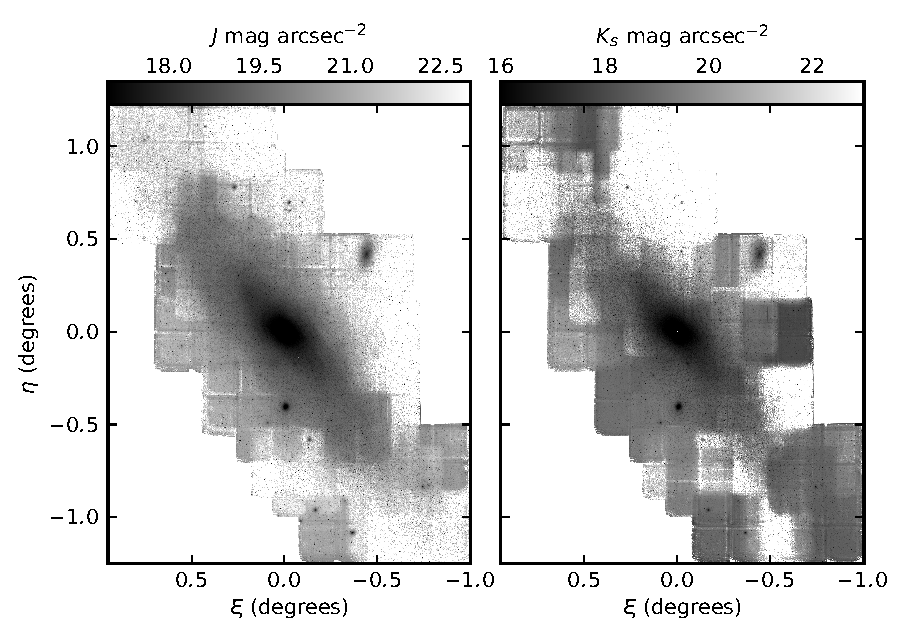
\includegraphics[width=3.5in]{figs/raw_mosaics}
	\caption{Median sky subtracted WIRCam $J$ (left) and $K_s$ (right) mosaics of M31.}
	\label{fig:raw_mosaics}
	% made with skysubpub/mosaic_plots.py
	% + skysubpub/raw_mosaic.py
\end{figure}

In Fig. \ref{fig:raw_mosaics} we plot mosaics (assembled using \sw{Swarp}) from \androids\ frames processed thus far. Although these basic image preparations dramatically improve image quality the \iiwione\ pipeline (particularly with regards to flat fielding performance), we see that classical NIR sky subtraction on a target as large as M31 is limited by an uncertainty of 1\% of the sky intensity. Classically, the true value of the sky on the disk of M31 is lost by the temporal and spatial variations of skyglow between disk and sky field observations.

% ============================================================================
\section{Scalar Sky Optimization}
\label{sec:scalar}

In this section, we demonstrate that the residual sky bias in each observation can be inferred from information in the overlaps of pairs of images in the mosaic. Each classically sky subtracted image of the M31 disk is a combination of the true surface intensity, $I_i$, and a residual sky intensity, $\epsilon_i$. Consider a pair of images, $i$ and $j$, that overlap on the galaxy: their difference is $(I_i+\epsilon_i) - (I_j+\epsilon_j) = \epsilon_i - \epsilon_j$. Given this measurement $\epsilon_i - \epsilon_j$ of residual sky intensity, we introduce \emph{sky offsets}, $\Delta$, for each observation so that

\begin{equation}
    (I_i + \epsilon_i - \Delta_i) - (I_j + \epsilon_j - \Delta_i) \rightarrow 0
\end{equation}

\noindent where the intrinsic intensities cancel, $I_i - I_j = 0$. Given a single pair of images, the inference of $\Delta_i$ and $\Delta_j$ is degenerate given the single difference image, $\epsilon_i-\epsilon_j$. But in a mosaic, each image is coupled (has overlapping domain) with many other images, and the mosaic itself can be considered as a network of coupled images. If we model the residual sky intensity $\epsilon_i$ as having a simple shape across the observed images, the single offset $\Delta_i$ will minimize all difference images involving image $i$. That is, sky offsets can be chosen by the non-linear optimization of

\begin{equation}
    \sum_{\forall i,j} [(\epsilon_i - \epsilon_j) - \Delta_i + \Delta_j] \rightarrow 0
    \label{eq:scalartheoryobj}
\end{equation}

\noindent over all coupled pairs $i,j$ in the mosaic.

This algorithm of introducing sky offsets that minimize the differences of all image pairs previously been implemented in the Montage mosaicing package \citep{Berriman:2008}. In that software, 1) images are rectified onto a mosaic pixel grid, 2) difference images are computed, and 3) sky offsets are iteratively chosen by looping through each image pair and choosing the offset needed to minimize the difference image of that pair, counting previous sky offset estimates. Rather than employ Montage for this M31 project, we were motivated to develop a new sky offset optimization algorithms for two reasons: to understand and improve the optimization convergence performance for a large data set, and to deeply understand the systematics and uncertainties of NIR sky subtraction residuals. Given the profound influence of sky residuals on the derived shape of M31's NIR disk, an assessment of uncertainty is crucial. An assessment of errors will be carried out in \todo{\S todo}. The convergence performance of sky optimization algorithms will be addressed in the proceeding sections.

\subsection{Hierarchical sky offset optimization}

Sky offset optimization is challenging because of dimensionality. Assuming that sky residuals are \emph{constant} across a frame (see \S TODO for the case of planar residuals), each image frame represents a new dimension ($\Delta_i$) in the optimization. Considering that the WIRCam array produces four image frames for every exposure, the combined 2007B and 2009B data sets consist of 3924 $J$ and 4972 $K_s$ image frames that cover the disk of M31. Such a large optimization is computationally ambitious, but also needless.

Our sky optimization algorithm breaks the optimization of sky offsets into three sequential steps, which we call \emph{hierarchical sky offset optimization}.

The 2007B and 2009B WIRCam surveys observed a total of 39 \emph{fields} across the M31 disk (illustrated in Fig. \ref{fig:fieldmap}). Each WIRCam field is imaged with four detectors, arranged in a $2\times 2$ grid. Let us define a \emph{detector field} as the collection of images that are taken with a given detector, at a given field. Images in a detector field have the greatly simplifying property of all overlapping across a dominant section of the image frame.

Thus in Step 1 we combine the frames in a detector field to produce a \emph{detector field stack}. The combined 2007B and 2009B surveys have 156 such stacks per filter. In Step 2, the four detector field stacks within each field can be fitted into a \emph{block}. A block is a fundamental unit of the mosaic, as all images that are combined within a block were observed under contemporaneous sky conditions. Finally, in Step 3, the 39 blocks can be fitted into a galaxy-wide mosaic for each filter.

\todo{Note how the certainty of sky offsets increases with the number of couplings}

\todo{Label the sky offsets that are produced in each step.}

\subsection{Construction of detector field stacks}
\label{sec:stacks}

Scalar sky offsets are most easily computed between the images of a detector field, since individual image frames in a detector field share a common footprint. That is, each image in a detector field is an (approximately) independent random estimate of the true surface brightness of the detector field. The mean surface brightness in the stack of images on a detector field is taken as the best estimate of the actual surface brightness. For each image frame, the difference between the surface brightness of the image and its best-estimate surface brightness of the detector field is taken scalar offset that brings the image to the level of the detector field stack.

The best estimate surface brightness for each detector field stack is first estimated as the mean-combination of all images in a detector field stack.  Since the telescope dithers by a few arcminutes between individual integrations, the edges of the detector field stack have a surface brightness that is estimated from a subset of all the images in a stack. The smaller ensemble of images leads to a visible bias at the stack's edges compared to the middle, where all frames contribute to the surface brightness estimation.

A solution is to estimate offsets for each frame compared to this first detector field stack. Offsets are computed as the median of the difference image between the stack and individual image frames, as described in \todo{Appendix on overlap detection}. The original image frames, now with offsets applied, are re-combined into a detector field stack image. Now edge-effects are smaller. Nonetheless, offsets are estimated a second time to produce a finalized detector field stack image.

\subsection{Non-linear optimization of block and mosaic sky offsets}

The detector field stacking phase (\S \ref{sec:stacks}) created high-\sn\ mosaics of the region covered by a given WIRCam detector at each survey field. Although these detector stacks are best estimates of the galaxy surface intensity at their regions, those stacks have systematic sky surface intensity uncertainties of $\sigma_s$. By combining stacks into blocks (step 2 of the hierarchical offset algorithm) and combining blocks in a mosaic (step 3), those uncertainties are diminished.

Unlike stack production, offsetting stacks into blocks and blocks into mosaics requires non-linear optimization since the images do not overlap simultaneously, but rather overlap in a network.

Let us define the objective function that encapsulates the effect of scalar sky offsets on reducing the intensity difference between coupled images:

\begin{equation}
    \mathcal{F} \left(\Delta_1,\ldots,\Delta_n \right) = \sum_{i,j} \mathcal{W}_{ij} \left( \langle \vect{I}_i - \vect{I}_j \rangle - \Delta_i + \Delta_j \right)^2,
    \label{eq:objf}
\end{equation}

\noindent which we intend to minimize by finding the optimal set of scalar sky offsets $\Delta_i$ for each of the detector fields $i$. Note that each coupled image pair is its own term in the objective summation, and that there are as many degrees of freedom ($\Delta_i$) as there are images in the mosaic. Each coupling is tempered by a weighting term $\mathcal{W}_{ij}$:

\begin{equation}
    \mathcal{W}_{ij} = \frac{A_{ij}}{\sigma_{\mathrm{\Delta ij}}},
\end{equation}

\noindent so that more priority is given to couplings of larger areas ($A_{ij}$), and small standard deviations of their difference images ($\sigma_{\Delta ij}$).

Note that the objective function in Eq. \ref{eq:objf} puts no constraint on the net sky offset: $\sum \Delta_i$. Assuming that sky subtraction errors are normally distributed, and not biased, sky subtraction offsets should not add a net amount of flux to the mosaic. Fortunately, it is possible to impose this constraint \textit{post facto} by subtracting the mean offset from the sky offsets:

\begin{equation}
    \Delta_i^* = \Delta_i - n^{-1}\sum_{j=1}^n \Delta_j.
    \label{eq:netzero}
\end{equation}

Given the image coupling records, I optimize the set of $\Delta_i$ using the \cite{Nelder:1965} (NM) downhill simplex algorithm. This NM algorithm has the advantage of being naturally multi-dimensional, and being able to work without knowledge of the gradient of the objective function. Instead, the NM algorithm operates by constructing a geometric simplex of $N+1$ dimensions that samples the sky offset parameter space. By evaluating the objective function at each vertex of the simplex, the NM algorithm adapts simplex's shape to ultimately contract upon a minimum.

But NM has two weaknesses. First, it is a \emph{greedy} optimizer that will converge into any local minimum, without necessarily seeking the global minimum. Second, for high-dimension optimizations (many fields in the mosaic), the NM may fail to converge in a reasonable number of objective function evaluations \citep{Neumann:2006}. Without solving these issues, a minimization of Eq. \ref{eq:objf} with an off-the-shelf NM code yields a mosaic with obvious discontinuities across fields. To solve the first problem, I develop a Multi-Start Reconverging NM (MSRNM) downhill simplex driver in Appendix \ref{cha:simplex}. This algorithm allows the NM to cumulatively cover a larger portion of parameter space to probabilistically ensure convergence into a global optimum.

% ============================================================================
\section{Analysis of Scalar Sky Offsets}
\label{sec:scalaranalysis}

\begin{itemize}
\item Figure \ref{fig:scalar_mosaics} --- maps
\item Table \ref{tab:offset_hierarchy} --- hierarchy of offsets
\item Figure \ref{fig:scalar_residual_sb_net} --- residual fluxes as surface brightness
\item Figure \ref{fig:scalar_relresidnet} --- residual fluxes compared to difference image uncertainties
\item Bootstrap to show uniqueness of solution (perhaps move this to section with comparison to Montage)
\end{itemize}

\begin{figure}[t]
	\centering
		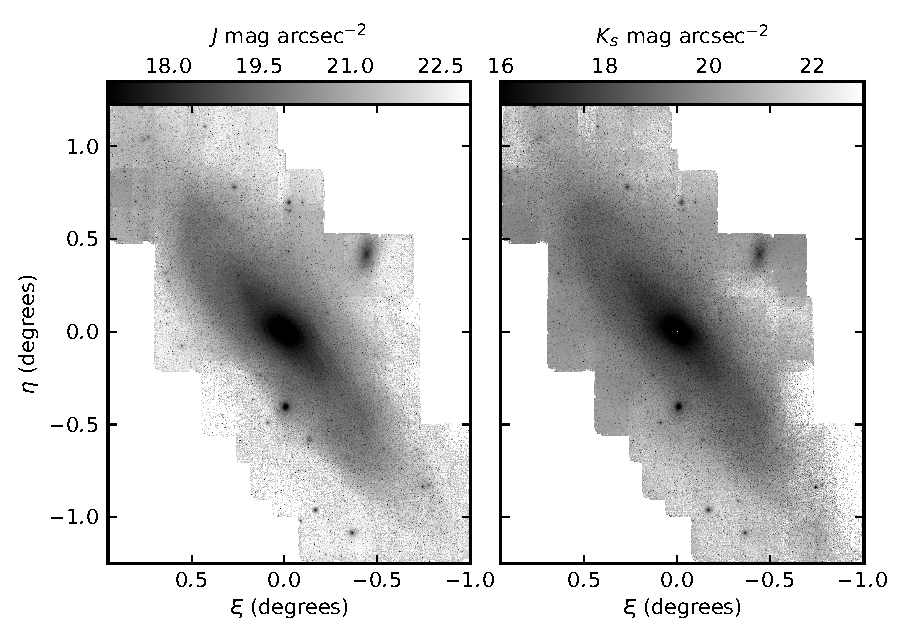
\includegraphics[width=3.5in]{figs/scalar_mosaics}
	\caption{Scalar-sky fitted WIRCam $J$ (left) and $K_s$ (right) mosaics of M31. Note the qualitative improvement compared to the original, median sky-subtracted, images in Fig. \ref{fig:raw_mosaics}.}
	\label{fig:scalar_mosaics}
	% made with skysubpub/mosaic_plots.py
\end{figure}

\begin{table}[t]
    \centering
    \caption[Hierarchy of scalar sky offsets]{Hierarchy of scalar sky offsets. The `Total' sky offsets track the net offset of individual WIRCam image frames into the fitted mosaic. $\langle I_\mathrm{sky}\rangle$ is taken as the typical instantaneous sky level for the images being sampled (see Fig. \ref{fig:net_sky_level} for the distribution of levels).}
% Fiducial sky values from thesis:
% J: $1.0\times 10^{-7}$ ADU s$^{-1}$ pix$^{-2}$
% K: $4.3\times 10^{-7}$ ADU s$^{-1}$ pix$^{-2}$
    \label{tab:offset_hierarchy}
% made with skyoffset/scalar_hierarchy.py
\begin{tabular}{ll|ll|ll}
% \hline
 &  & \multicolumn{2}{c|}{$J$} & \multicolumn{2}{c}{$K_s$} \\ % \cline{3-4} \cline{5-6}
% \hline
Offset Type & Sem. & $\sigma_\Delta$ & $\frac{\sigma_\Delta}{\langle I_\mathrm{sky}\rangle }$ & $\sigma_\Delta$ & $\frac{\sigma_\Delta}{\langle I_\mathrm{sky}\rangle }$ \\
 & & \tiny{(mag~arcsec$^{-2}$)} &  \tiny{(\%)} & \tiny{(mag~arcsec$^{-2}$)} &  \tiny{(\%)} \\
\hline
\multirow{2}{*}{Frame to stack} & 07B & 20.1 & 1.02 & 18.1 & 1.37 \\
% \hline
 & 09B  & 20.4 & 0.42 & 18.2 & 1.04 \\
\hline
\multirow{2}{*}{Stack to block} & 07B & 22.4 & 0.11 & 21.2 & 0.09 \\
% \hline
  & 09B & 24.2 & 0.01 & 22.2 & 0.03\\
\hline
\multirow{2}{*}{block to mosaic} & 07B & 20.8 & 0.54 & 19.0 & 0.55 \\
% \hline
  & 09B & 21.3 & 0.19 & 19.2 & 0.43 \\
% \hline
\hline
\multirow{2}{*}{Total} & 07B & 19.9 & 1.16 & 18.0 & 1.49 \\
% \hline
  & 09B & 20.3 & 0.48 & 18.1 & 1.12 \\
% \hline
\end{tabular}
\end{table}

% made with skyoffset/scalar_hierarchy.py
% type Band, Semester, mag sigma, sigma/sky
% frame J 2007 20.0 1.02
% frame J 2009 20.4 0.42
% 
% stack J 2007 22.4 0.11
% stack J 2009 24.2 0.01
% 
% block J 2007 20.8 0.54
% block J 2009 21.3 0.19
% 
% total J 2007 19.9 1.16
% total J 2009 20.3 0.48
% --
% frame K 2007 18.1 1.37
% frame K 2009 18.2 1.04
% 
% stack K 2007 21.2 0.09
% stack K 2009 22.2 0.03
% 
% block K 2007 19.0 0.55
% block K 2009 19.2 0.43
% 
% total K 2007 18.0 1.49
% total K 2009 18.1 1.12

\begin{figure}[t]
    \centering
        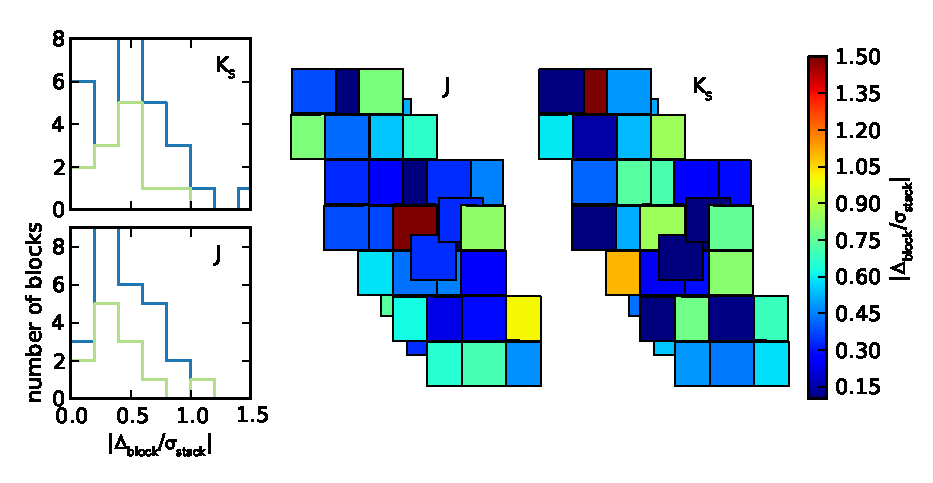
\includegraphics[width=3.5in]{figs/offset_ratio_map_enhanced}
    \caption{Acceptability of $J$ and $K_s$ scalar sky offsets between blocks, as measured by the ratio of $\Delta_\mathrm{block}/\sigma_\mathrm{stack}$.}
    \label{fig:offset_ratio_map}
    % made with skyoffset/offsetratiomap.py
    % TODO need to fix colour scheme of the histograms
\end{figure}

\begin{figure}[t]
    \centering
        \includegraphics[width=3.5in]{figs/scalar_residual_sb_net}
    \caption{Residual surface brightness differences after scalar fitting.}
    \label{fig:scalar_residual_sb_net}
    % made with skyoffset/networkmap.py
    % TODO need to fix colour scheme of the histograms
\end{figure}

\begin{figure}[t]
    \centering
        \includegraphics[width=3.5in]{figs/scalar_relresidnet}
    \caption{Residual surface brightness differences relative to the intensity uncertainty of the coupled difference images.}
    \label{fig:scalar_relresidnet}
    % made with skyoffset/networkmap.py
    % TODO need to fix colour scheme of the histograms
\end{figure}

% ============================================================================
\section{Planar Sky Offsets}

Scalar sky offsets are greatly effective for recovering the galaxy intensity from sky background uncertainties. But the reconstructed galaxy mosaics (Fig. \todo{maps}) reveal field-to-field discontinuities in the outer disk of roughly the same magnitude as the intrinsic disk surface brightness. These discontinuities are not a failure of the scalar sky offset method to converge; rather, they reveal that residual sky flux has a \emph{shape} across blocks.

Figure \todo{horizontal cut} shows cuts of surface intensity across the $K_s$ scalar-sky corrected mosaic. \todo{Comment on the figure, that blocks have slopes that are not continuous}.

Importantly, these residual sky shape are discontinuous only \emph{between} blocks. Figure \todo{todo} shows surface intensity cuts the component stacks of blocks. None of the blocks show surface intensity breaks between stacks. Recall that stacks within a block are simultaneously observed so that the residual sky present in each stack is correlated. In Table \ref{offset hierarchy table} we realized that $\Delta_\mathrm{stack}$ offsets are minor, and again, we see that sky shape discontinuities within blocks are negligible.

This implies that any endeavor to removed residual sky shapes in the final mosaic need only operate at the block level: scalar sky offsets are an acceptable method for \emph{producing} blocks. In this section would outline such a method where we assume that residual sky shapes can be modeled as planes across blocks. This assumption is consistent with out need to be economical in the dimensionality of optimizations. Since a plane is parameterized as two slopes an a level, the optimization of 39 blocks in each M31 mosaic requires 117 parameters.

\subsection{Planar Sky Offset Optimization Algorithm}

Our planar sky offset optimization algorithm is a direct evolution of the scalar case. As before, difference images are assembled from each coupled pair of blocks. For each difference image we fit a plane $\epsilon_{ij} = (m_x, m_y, c)$: that is, $x$- and $y$-axis slopes and the level $c$ at the center of the difference image. The plane fitting is done iteratively with sigma clipping to reduce the influence of stellar PSF differences of bright stars. Our goal is now to find the sky offset planes for each block, $\Delta_\mathrm{block} = (\Delta_x, \Delta_y, \Delta_c)$, that maximally reduce flux in the difference planes.

The multi-start re-converging Nelder-Mead simplex is again a flexible tool for searching parameter space and finding a global minimum. Planar optimization is more challenging because the parameters in the simplex no longer carry the same meanings, and in particular, have different dynamic ranges. Though we attempted to simultaneously optimize planar slopes and levels by scaling slopes to the same order as levels, that optimization apparatus never converged reliably. Instead, we use an algorithm that iteratively alternates between improving planar levels and slopes until convergence is reached.

Working in the framework of a multi-start optimization, we generate a large suite of random planar offsets that serve as starting points for each optimization `start.' Random planar offsets have levels and slopes drawn from Gaussian distributions $N(0, \sigma_{c,\mathrm{init}})$ and $N(0, \sigma_{x,y,\mathrm{init}})$, respectively. From each initial point, the optimization two Nelder Meade simplex optimizations in succession, each with the ensured reconvergence mechanism (previously described for scalar offset optimization \S \todo{todo}).

First, planar slopes are optimized. The objective function considers only the minimization of slopes in the difference planes:

\begin{equation}
	\mathcal{F}_m(m_x^0,m_y^0,\ldots m_x^n, m_y^n) = \sum_{i,j} \epsilon_x^{ij} - \Delta_x^i - \Delta_x^j + \epsilon_y^{ij} - \Delta_y^i - \Delta_y^j
\end{equation}

\noindent As done in scalar offset optimization, any converged solution for the best slopes is restarted and reconverged until a stable minimum of the objective function is found (see \S \todo{restart mechanism}).

Second, the overall levels of offset planes are optimized. This objective function takes the offset slopes derived in the previous step, and seeks to minimize the level, $\epsilon_c$, of difference planes' centers:

\begin{eqnarray}\nonumber
	\mathcal{F}_c(\Delta_\mathrm{block}^0,\ldots,\Delta_\mathrm{block}^n) = &\sum_{i,j}& \mathcal{W}_{ij} [ \epsilon^{ij}_c - (\Delta_c^i + D_x^i\Delta_x^i + D_y^i\Delta_y^i) \\
	&& +~(\Delta_c^j + D_x^j\Delta_x^j + D_y^j\Delta_y^j) ]
\end{eqnarray}

$D_x$ and $D_y$ are distances from the center of the offset plane $\Delta$ to the center of the difference image $\epsilon_ij$. Thus $D_x\Delta_x$ and $D_y\Delta_y$ terms account for the slope's effect on the offset planes level at the center of the $\epsilon_{ij}$ difference image. Again, the restart mechanism is used to ensure a robust minimum of the $\mathcal{F}_c$ objective function.

Together, these two optimization steps produce a new generation of $\Delta_\mathrm{block}$ planar offsets. These new offsets are compared to the previous generation (or the initial random planes for the first iteration) and the fractional difference of each slope and offset is measured. If any fractional difference exceeds a convergence tolerance of 10$^{-7}$, another iteration of optimization is performed. In this iteration, the current planes become new seed planes, and the successive slope and level optimizations are performed. Once an iteration produces planes effectively identical to the previous iteration, the optimization is stopped.

The $N$ optimization starts creates $N$ potential sky offset solutions. To choose the best solution, we seek the solution that minimized the level objective function, $\mathcal{F}_c$. This objective is sensitive to the overall surface intensity difference between coupled fields, while still being dependent on the quality of the planar slopes.

Optimized planar offsets can add a arbitrary amount of flux to a mosaic, and this net offset must be subtracted. Both the net levels and net slopes of the offset planes be subtracted. Given the set of optimized offset planes, $\Delta$, a \emph{net offset plane} $p$ can be constructed:

\begin{eqnarray}
	p_x & = & n^{-1} \sum_{i=0}^n \Delta_x^i \\
	p_y & = & n^{-1} \sum_{i=0}^n \Delta_y^i \\
	p_c & = & n^{-1} \sum_{i=0}^n \Delta_c^i
\end{eqnarray}

\noindent This net offset plane is subtracted from each optimized offset plane to obtain the final set of planar sky offsets for blocks in the mosaic.

\subsection{Analysis of Planar Sky Offsets}

\begin{itemize}
	\item Figure \ref{fig:planar_mosaics} --- mosaics made with planar optimization
	\item Distribution of planar slopes
	\item Residual network plot
\end{itemize}

\begin{figure}[t]
	\centering
		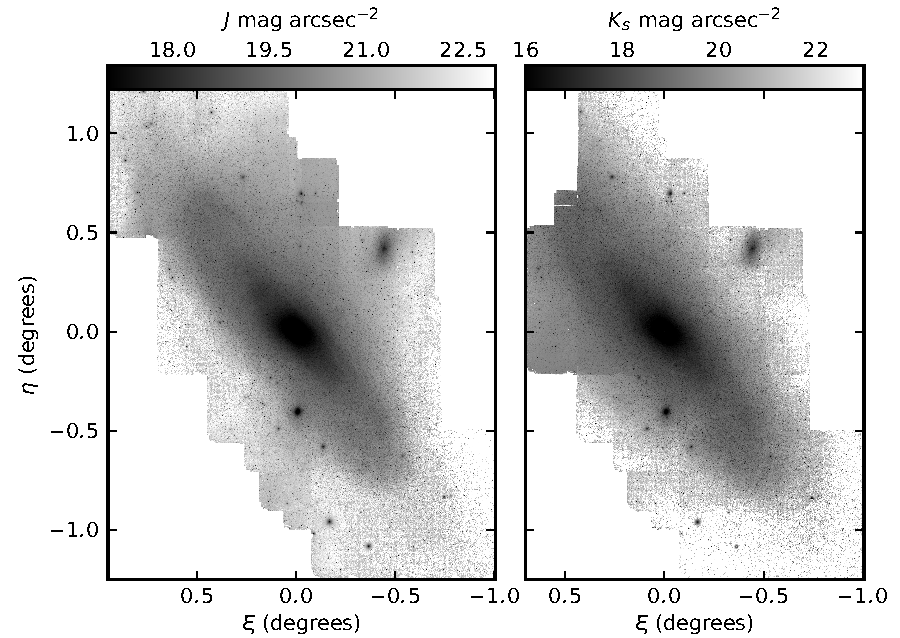
\includegraphics[width=3.5in]{figs/planar_mosaics}
	\caption{Planar sky fitted WIRCam $J$ (left) and $K_s$ (right) mosaics of M31.}
	\label{fig:planar_mosaics}
	% made with skysubpub/mosaic_plots.py
\end{figure}

% ============================================================================
\section{Systematic Uncertainties in Surface Brightness Reconstruction}
\label{sec:systematics}

\begin{figure}[t]
    \centering
        \includegraphics[width=3.5in]{figs/sbdiff/scalar_irac36_sbdiff.pdf}
    \caption{Maps of $J-[3.6]$ and $K_s-[3.6]$ surface colour inferred from the scalar-sky fitted WIRCam mosaics (see \S\ref{sec:scalar}--\ref{sec:scalaranalysis}) and Spitzer/IRAC 3.6~$\mu$m image \citep{Barmby:2006}. Note that the IRAC map crops the \androids/WIRCam footprint.}
    \label{fig:scalar_irac36_sbdiff}
    % make with skysubpub/diffplots.py
\end{figure}

\begin{figure}[t]
    \centering
        \includegraphics[width=3.5in]{figs/sbdiff/altplanar_irac36_sbdiff.pdf}
    \caption{Maps of $J-[3.6]$ and $K_s-[3.6]$ surface colour inferred from the planar-sky fitted WIRCam mosaics (see \S\ref{sec:scalar}--\ref{sec:scalaranalysis}) and Spitzer/IRAC 3.6~$\mu$m image \citep{Barmby:2006}. Note that the IRAC map crops the \androids/WIRCam footprint.}
    \label{fig:altplanar_irac36_sbdiff}
\end{figure}

Sky offsets produce a mosaic that is rigorously optimal only in the sense of field-to-field surface brightness continuity---not absolute sky subtraction. In this section, we attempt to gauge the systematic surface brightness error inherent in the sky offset technique.

\subsection{Comparison to Spitzer/IRAC Images}

Systematic uncertainties can be explored by comparing our WIRCam mosaics to well-calibrated images of M31, and looking for colour discrepancies.
A template for the old stellar disk, is the 3.6~$\mu$m Spitzer/IRAC map, presented in \cite{Barmby:2006}, which avoids sky subtraction uncertainties inherent in ground-based observation.
In Fig. \ref{fig:scalar_irac36_sbdiff} we compare the scalar-fitted mosaics against the 3.6~$\mu$m image. Generally the $J-[3.6]$ and $K_s-[3.6]$ colors decrease with disk radius, but increase in the star-forming regions because of hot dust emission. Both the scalar-fitted $J$ and $K_s$ mosaics are reddened in the south-eastern corner, which we interpret as a systematic \emph{over-subtraction} of the WIRCam NIR sky. In $J-[3.6]$ and $K_s-[3.6]$ maps realized with planar-fitted sky, Fig. \ref{fig:altplanar_irac36_sbdiff}, a similar, though stronger, systematic sky error is seen. This result qualitatively illustrates the greater potential for systematic sky errors when planar sky correction freedom is permitted across the $20\times 20$ arcmin WIRCam blocks.

\subsection{Comparison to \sw{Montage}-fitted images}

\begin{figure}[t]
    \centering
        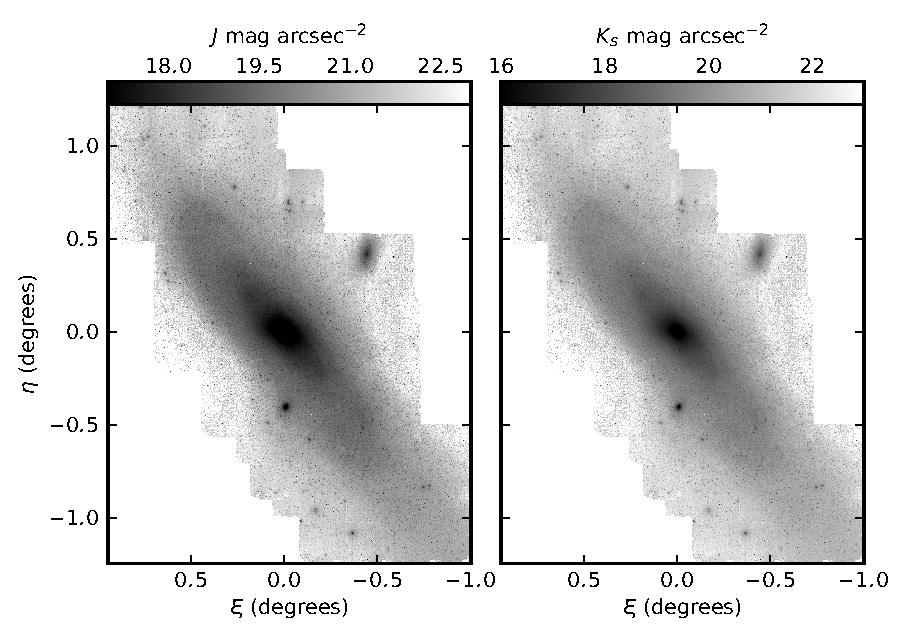
\includegraphics[width=3.5in]{figs/montage_planar_mosaics.pdf}
    \caption{Montage-generated $J$ and $K_s$ maps. Compare to the equivalent simplex maps, Figs. \ref{fig:scalar_mosaics} and \ref{fig:planar_mosaics}. Pixels with negative surface intensity, after sky offset correction, are masked with white.}
    \label{fig:montage_planar_mosaics}
    % make with skysubpub/mosaic_plots.py and skyoffset/montageoffsets.py
\end{figure}

\begin{figure}[t]
    \centering
        \includegraphics[width=3.5in]{figs/sbdiff/montage_irac36_sbdiff.pdf}
    \caption{Maps of $J-[3.6]$ and $K_s-[3.6]$ surface colour inferred from the \sw{Montage}-fitted WIRCam mosaics (see Fig. \ref{fig:montage_planar_mosaics}).}
    \label{fig:montage_irac36_sbdiff}
    % make with skysubpub/diffplots.py
\end{figure}

\begin{figure}[t]
    \centering
        \includegraphics[width=3.5in]{figs/sbdiff/altplanar_jk_sbdiff.pdf}
    \caption{$J-K_s$ colour maps realized by the simplex planar sky fitting algorithm (left) and \sw{Montage} (right).}
    \label{fig:altplanar_jk_sbdiff}
    % make with skysubpub/diffplots.py
\end{figure}


Although this paper advocates a sky offset optimization based on the \cite{Nelder:1965} Downhill Simplex algorithm, other tools exist for solving sky background corrections. A popular package is \sw{Montage} \citep{Berriman:2008}. Like the algorithms presented in this paper, \sw{Montage} uses the network of image-to-image differences to infer sky offsets. Rather than simultaneously solve for all offsets, \sw{Montage} uses an iterative algorithm: offsets are proposed that arithmetically solve one pair of images, and that offset change is propagated into the adjacent pair, which are again arithmetically offset, and so forth.

Figure \ref{fig:montage_planar_mosaics} shows mosaics generated by \sw{Montage}, allowing for planar sky offsets. These surface brightness realizations lead to $J-[3.6]$ and $K_s-[3.6]$ maps in Fig. \ref{fig:montage_irac36_sbdiff}. Comparing the simplex-optimized color map (Fig \ref{fig:altplanar_irac36_sbdiff}) against the \sw{Montage} realization, it is plain that the two algorithms find different sets of globally optimum sky offsets. And neither of the solutions is optimal in the sense of absolute calibration.

Another useful comparison is Figure \ref{fig:altplanar_jk_sbdiff}, where $J-K_s$ color maps are realized by both the simplex planar-fitting and \sw{Montage} algorithms. Unlike the comparisons against $[3.6]$, these color maps test the entire \androids\ footprint. Absolute calibration of the NIR surface brightness is a clear requisite before these images are scientifically useful beyond the inner disk.

\subsection{Bootstrap analysis of systematic surface brightness uncertainties}

\begin{figure}[t]
    \centering
        \includegraphics[width=3.5in]{figs/bootstrap_sb_rms.pdf}
    \caption{Maps of bootstrap RMS surface brightness in $J$ (left) and $K_s$ (right) mosaics. White contours identify RMS levels of 0.05 (solid), 0.1 (dashed) and 0.2 (dash-dot) mag arcsec$^{-2}$.}
    \label{fig:bootstrap_sb_rms}
    % made with skyoffset/bootstrap.py BootstrapRMSPlot
\end{figure}

\begin{figure}[t]
    \centering
        \includegraphics[width=3.5in]{figs/bootstrap_recovery_map.pdf}
    \caption{Dispersions ($1\sigma$) in the difference of expected and observed sky offsets in bootstrap realizations of the $J$ (left) and $K_s$ (right) mosaics. The 2009B fields are plotted over top of the 2007B fields (see Fig. \ref{fig:fieldmap} for spatial reference).}
    \label{fig:bootstrap_recovery_map}
    % made with skyoffset/bootstrap.py OffsetRecoveryFieldMap
\end{figure}


The difference images presented in the previous section, and particularly Fig \ref{fig:altplanar_jk_sbdiff}, illustrate how the surface brightness reconstructions of identical data can vary depending on the optimization algorithm. Here we pose a slightly different question: how are reconstructions affected by the initial conditions of sky errors? We answer this with a bootstrap analysis.

A bootstrap realization is generated by perturbing the surface brightness of the corrected blocks with a sky error drawn (with replacement) from the ensemble of block sky offsets observed in the original mosaic (Fig. \ref{fig:scalar_mosaics}). Using the scalar-sky fitting procedure, sky offsets  are optimized against the known sky perturbations. 150 such realizations are made to compile an ensemble of mosaics in both bands.

Figure \ref{fig:bootstrap_sb_rms} shows the RMS deviation of bootstrapped mosaic surface brightness against the original scalar-fitted mosaics. Reconstructed surface brightness in the outer disk can vary $\sim 1$ mag arcsec$^{-2}$, consistent with colour biases in the $J-[3.6]$ and $K_s-[3.6]$ maps.

Another view into this effect is Fig. \ref{fig:bootstrap_recovery_map}, where the standard deviations between expected and realized sky bootstrap offsets is plotted. These maps show that the typical error in realized offset, compared to input sky perturbation, is 0.05\%--0.10\% of the sky intensity. One hypothesis is that this sky offset recovery error is due to flexure in the mosaic---where blocks on the mosaic periphery are forced to conform to the surface brightness of more central and tightly coupled blocks. Yet Fig. \ref{fig:bootstrap_recovery_map} does not show a clear outside-in trend. The $J$ map (Fig.~\ref{fig:bootstrap_recovery_map} [left]) does show a slight north-south trend, but more abundant is the precision with with sky perturbations for the 2009B fields were recovered.

Rather than mosaic flexure, a better model for Fig. \ref{fig:bootstrap_recovery_map} is uncertainties in the \textit{post priori} adjustment for zero net offset (Eq.~\ref{eq:netzero}). Since block sky offsets have approximately Gaussian distributions with dispersions given in Table \ref{tab:offset_hierarchy}, the uncertainty in the net offset correction is simply $\sigma(\mathrm{block})/\sqrt{n_\mathrm{blocks}}$. Considering the dispersions among 2007B block offsets, the expected uncertainty of the zero net offset correction is 0.08\% and 0.09\% of the $J$ and $K_s$ sky intensity, respectively. The dominant source of uncertainty shown in the bootstrap simulations, Figs. \ref{fig:bootstrap_sb_rms} and \ref{fig:bootstrap_recovery_map}, is the use of an arithmetic mean of offsets to set an absolute zeropoint, not flexure or uncertainty in the network of offsets. This suggests that external zeropoints could be very useful in replacing Eq.~\ref{eq:netzero}. Since no absolutely-calibrated NIR photometry of M31's surface brightness exists, we will discuss a method using panchromatic resolved stellar populations in a future work.

% ============================================================================
\section{Conclusions}
\label{sec:conclusions}

\bibliography{master}

\end{document}
